\section{Results}
\label{sec:results}

The primary experiment is the Class~A search for a drifting, unresolved
spectral carrier: \NWinA{} fine-channel windows toward \NSysClassA{}
systems. The Class~B search for an unresolved spectral excess is secondary
and carries no drift discrimination: \NWinB{} coarse windows. Together they
are the \NWindows{} windows of the released catalogue. \textbf{No event
satisfied the confirmation criterion set out in \S\ref{sec:summary}.} What
follows is first how deep the search reaches, and then what it found and how
each finding was disposed of.

\subsection{Sensitivity: the power at which a carrier would have been
found} \label{sec:pninetysel}

\emph{The sensitivity of this survey is a measured completeness and not a
threshold.} Artificial carriers were added to the real calibrated
visibilities at a random sub-channel phase and a random drift from each
window's own grid and recovered through the unchanged pipeline; the power at
which nine in ten come back is $\mathrm{EIRP}_{90}$, the only sensitivity
quoted here. \emph{It is measured through the chain the survey applies} ---
the trigger and localisation at the stellar position. The \NCtrl-position
spatial rank annotates a crossing rather than deciding it
(\S\ref{sec:summary}) and is not charged against it: it would cost a further
factor $\SensCostLike$ and in \SensNRingHiUnres{} bright-ring windows could
not be met at any injected power (Fig.~\ref{fig:strata}), and a limit should
not be charged for a gate that disposes of nothing.

\emph{Measured that way the completeness is one number.} Nine carriers in ten
are recovered at $\SensMultA\,P_{\rm trig}$, where $P_{\rm trig}$ is the
window's own trigger power, and that class-average factor is determined to
$\pm\SensBootPct$ per cent. Every one of the \SensNInj{} directly injected
Class~A windows resolves a ninety per cent point of its own, between
$\SensIndivLo$ and $\SensIndivHi\,P_{\rm trig}$, and the value does not
depend on the brightness of the window's control ring: the \SensNRingHi{}
windows whose ring carries resolved emission come back at
$\SensRingHi\,P_{\rm trig}$ against $\SensRingLo$ for the rest
(Fig.~\ref{fig:strata}). One factor therefore serves the class. Class~B
carries
its own factor $\EirpNinetyMultB\,P_{\rm trig}$, measured the same way from
\SensNToneCoarse{} carriers injected into \SensNInjCoarse{} coarse windows of
\SensNInjCoarseBlock{} execution blocks and weighted by the coarse
catalogue's own distribution of ring brightness; it is what sets the limits
for Barnard's Star, Wolf~359 and Proxima.

\emph{The resulting limits.} The median Class~A window reaches
$\EirpNinetyWinMedA$\,W of equivalent isotropic radiated power and the median
system, on its best window, $\EirpNinetySysMedA$\,W, with a spread across
systems of $\EirpNinetySysLoA$--$\EirpNinetySysHiA$\,W
(Fig.~\ref{fig:classasens}a). The round $10^{15}$\,W level is reached for
\NSysEfifteen{} of them. Table~\ref{tab:p90budget} collects the terms acting
on those numbers. The calibration of the factor is good to
$\times\SensFacLo$--$\times\SensFacHi$, and that is the interval which
applies to the median and to the counts. One bias is not inside it and runs
one way only: an injected carrier is added to visibilities that have already
been calibrated and so suffers no atmospheric or instrumental decorrelation,
whereas a real carrier does, so \textbf{every limit in this paper is
optimistic by up to \SensDecorPct{} per cent} on that account --- a figure
declared from the literature rather than measured here.

\emph{Carriers were injected directly into \SensNInj{} of the \NWinA{}
Class~A windows, \SensNInjPct{} per cent, and the result transferred to the
remaining \SensNTransfer, which is the dominant caveat on all of the above.}
The injected windows are the Class~A windows of execution blocks drawn in a
stratified random order fixed in advance, without reference to which windows
hold a crossing; they hold \SensNCrossAch{} crossings against the
\SensNCrossExp{} the population rate predicts. \emph{The unit is the block
and not the window}, because a block's calibrated visibilities are what an
injection campaign has to rebuild: band and array were controlled by the
draw, while channel width, ring brightness and integration length vary inside
a block and were only compared with the population afterwards, agreeing to
\SensCovWorstPct{} per cent on the worst axis.

\emph{Every limit therefore rests on the class-average calibration, and what
one window may differ from it by is a separate statement.} The median ninety
per cent point differs by \SensBandSpread{} between bands,
\SensChanSpread{} between channel widths and \SensArrSpread{} between the two
arrays. The largest of the three is the \SensCovAxis, and none of them is as
large as the gate the chain no longer charges for. The array difference
survives setting the bright-ring windows aside --- \SensArrSpreadFaint{}
without them --- so it belongs to the array and not to its fields, as a
compact array keeping more extended emission inside its beam would.
Across the injected windows as
a whole the ninety per cent point ranges from $\times\SensIndivFacLo$ to
$\times\SensIndivFacHi$ of the adopted factor, so an individual uninjected
window's own completeness is not known to the precision of the interval that
applies to the class.

\emph{One geometric term acts window by window, and it is measured rather
than modelled.} The phase centre assumed in the search omits the annual
parallax, which displaces the star by a median \SensBeamsMed{} of a
synthesised beam and at most \SensBeamsMax. Each limit is therefore divided
by the amplitude a compact source retains at its own displacement --- read
off an injection into the same visibilities at both positions, not off a beam
model (Appendix~\ref{app:conventions}) --- which makes the median Class~A
limit shallower by \PxaShiftWinPct{} per cent. One window,
\PxaMissingStar{} in \PxaMissingEb, has no astrometric keys and is left
uncorrected.

\emph{A carrier that is not always radiating is penalised in proportion.} The
de-drifted stack is coherent across a whole execution block, so a carrier
present for a fraction of one contributes to that fraction of the
integrations and comes back at that fraction of its continuous amplitude.
Over \DutyNTrial{} trials in \DutyNWin{} windows of \DutyNStar{} stars, at
\DutyNCycle{} duty cycles within a track down to \DutyCycleMinPct{} per cent
and at amplitudes between $\times\DutyAmpTrigLo$ and $\times\DutyAmpTrigHi$
of each window's own trigger, the recovered amplitude followed the duty cycle
to \DutyAttenDevPct{} per cent. A transmitter radiating a tenth of the time
therefore needs $\DutyPowFac\times$ the power quoted above, and because those
trials carry no drift the joint drifting and intermittent case is not
measured here at all.

\begin{table}
\centering
\scriptsize
\caption{What sets $\mathrm{EIRP}_{90}$, and in which direction. The
uncertainty on the calibration is an uncertainty on the class-average factor,
and so on any statistic formed over many windows; the spread between windows
is an observed dispersion and is the statement about one window's own limit;
the signed terms are biases, stated with their direction rather than folded
into an error bar. The channel response is carried by the injections rather
than applied afterwards, so it must not be applied again
(Appendix~\ref{app:conventions}).}
\label{tab:p90budget}
\tiny
\setlength{\tabcolsep}{2pt}
% GENERATED by sens_r11.py -- do not hand-edit.
\begin{tabular}{@{}l@{~~}r@{~~}>{\raggedright\arraybackslash}p{0.37\columnwidth}@{}}
\hline
 & value & what it does to the limit \\
\hline
Class-average completeness & $\times3.03$ & nine carriers in ten recovered at this multiple of a window's own trigger power, over 49 injected Class~A windows \\
\hline
\multicolumn{3}{@{}l}{\emph{Uncertainty on that calibration} (per cent), combined in quadrature} \\
The factor itself & $\pm2$ & sampling error of the pooled value over the 49 injected windows \\
Flux, distance and visibility scale & $\pm9$ & calibration \\
\emph{Combined} & $-9/+9$ & $\times0.91$--$\times1.09$ on the factor, and so on the median limit and on the system counts \\
\hline
\multicolumn{3}{@{}l}{\emph{Spread between windows}. An observed dispersion, not an error bar.} \\
Window to window & $\times0.80$--$\times1.58$ & the 49 injected windows resolve 2.41--4.80\,$P_{\rm trig}$ individually, so an uninjected window's own completeness is not known to the interval above \\
\hline
\multicolumn{3}{@{}l}{\emph{Signed terms}. A bias is not an error bar and is not added to one.} \\
Channel response & $\times\InjPeakAtNinety$ & carried by the injections, so already inside the completeness above \\
\quad its residual & $+\InjShortPct$ & the injected profile falls short of the exact response: \emph{conservative} \\
Primary-beam model & $+0/+10$ & ALMA's beamwidth in place of the pipeline's Airy-null one: nothing in the median window, 4 windows of one star \\
Decorrelation & $+0/+20$ & an injected carrier suffers none and a real one does, so every limit is optimistic by up to this much; declared from the literature, not measured here \\
\hline
\end{tabular}

\end{table}

\begin{figure}
\centering
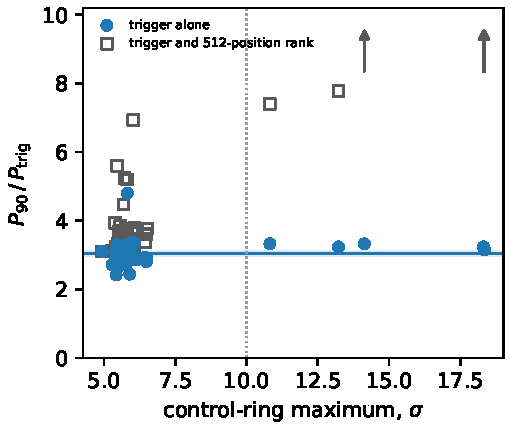
\includegraphics[width=0.96\columnwidth]{figures/sens_ring.pdf}
\caption{Why one completeness factor serves the whole class. Each of the
\SensNInj{} directly injected Class~A windows is plotted at the power that
recovers nine carriers in ten, against the maximum of its own
\NCtrl-position control ring. Filled circles are the criterion adopted
here --- the trigger and localisation at the star --- with the pooled value
and its uncertainty as the line and band; they show no trend with the ring.
Open squares add the demand that the carrier outrank every control position,
and arrows mark the windows that then reach ninety per cent at no injected
power. Dotted, the $\SensRingRule\sigma$ ring brightness above which a ring
carries resolved emission rather than noise.}
\label{fig:strata}
\end{figure}

\begin{figure*}
\centering
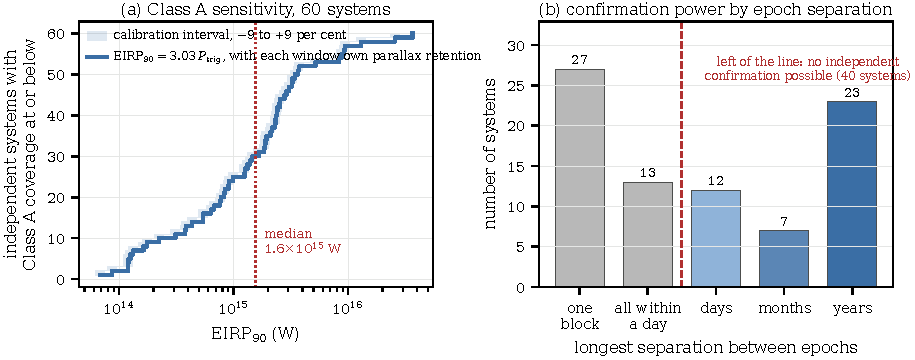
\includegraphics[width=0.92\textwidth]{figures/classa_sensitivity.pdf}
\caption{\emph{(a)}~Class~A sensitivity: the cumulative number of systems
whose best window reaches a given $\mathrm{EIRP}_{90}$, the power at which
nine carriers in ten are recovered through the trigger at the star. Every
window is drawn on the one adopted convention,
$\SensMultA\,P_{\rm trig}$ with that window's own annual-parallax retention
applied, and the shaded band is the calibration interval of
Table~\ref{tab:p90budget}. \emph{(b)}~The temporal selection function:
systems grouped by the longest separation between their searched epochs, an
independent epoch being a separation of more than \EpSep{} day.
\textbf{For the \EpOne{} systems observed in a single block, and the
\EpSameDay{} whose blocks all fall within one day --- left of the dashed
line --- independent confirmation was not possible at all}, whatever the
sensitivity in panel~(a).}
\label{fig:classasens}
\end{figure*}

\subsection{The nearest stars: Barnard's Star and Wolf~359}
\label{sec:barnardswolf}

Barnard's Star is the second-nearest stellar system and Wolf~359 the third if
brown dwarfs are excluded, and to our knowledge these are the first millimetre
or submillimetre technosignature limits for either \citep{Enriquez2017,
Price2020, Margot2023}. Both are non-detections. \emph{Both limits come from
the secondary Class~B experiment and not from the carrier search}: the archive
holds only coarse Band~6 windows toward these stars, so what is constrained is
an unresolved spectral excess and not a drifting carrier. On the
$\mathrm{EIRP}_{90}$ convention of \S\ref{sec:pninetysel} Barnard's Star
reaches $\EirpNinetyBarnLo$--$\EirpNinetyBarnHi$\,W over \NWinBarn{} windows
and Wolf~359 $\EirpNinetyWolfLo$--$\EirpNinetyWolfHi$\,W over \NWinWolf.

\subsection{Threshold crossings and how each was disposed of}
\label{sec:technosearch}

\emph{The result is a chain of three tests, and it is read in one direction.}
Of the \NWindows{} windows, \EvNCrossRaw{} contain a
channel\,$\times$\,drift cell at the stellar position reaching $T\geq5$, and
such a cell is a \emph{threshold crossing}. \EvNCrossFlag{} lie in the one
execution block that fails the quality criterion of \S\ref{sec:bdblock},
fixed before it was applied, so the population characterising the search is
the \EvNCrossQp{} crossings in quality-passing data and those
\EvNCrossFlag{} are reported beside it rather than within it. The
molecular-line mask,
$\pm\MaskHalfKms$\,km\,s$^{-1}$ wide and evaluated in each star's own rest
frame, identifies \EvNAttrQp{} of the \EvNCrossQp{} with a catalogued
transition and leaves \EvNUnattrQp{} unattributed; every crossing is in one
column or the other. Of the unattributed, \EvNRankQp{} outrank all
\NCtrl{} control positions of their own window, and neither recurs in any
later epoch covering its frequency. \textbf{No crossing survives the chain,
and this survey reports no detection.}
Figure~\ref{fig:chain} carries the chain with the number surviving each
step and Tables~\ref{tab:ledger} and~\ref{tab:ledgercont} the
crossing-by-crossing ledger behind it.

\emph{The mask is informative rather than permissive, and its half-width
follows from the Keplerian velocity bound on circumstellar gas in these
systems rather than from tuning} (Appendix~\ref{app:linemask}). The
attributions are kinematic and not an accident of bandwidth, and the
comparison that shows it is per window and not over the union band: of the
\AppMNCrossF{} crossings for which the release records a measured peak
frequency, \AppMTubeObs{} fall within $\pm\DispoHalfKms$\,km\,s$^{-1}$ of a
searched transition against \AppMTubeNull{} expected were each peak free to
land anywhere on its own window's channel grid (Appendix~\ref{app:rfi}).

\subsubsection{Most of the crossings are expected by chance}
\label{sec:trigunif}

The trigger is a threshold on a statistic and not a false-alarm rate: the
number of searched channel\,$\times$\,drift cells per window spans
\TuCellsDecades{} decades, so one level buys very unequal protection. How
many crossings chance should produce is therefore measured window by window,
with the same selection on both sides of the comparison --- the \NWinA{}
Class~A windows of the census, and in each of them a cell at the stellar
position reaching the trigger which the line mask does not attribute. A
window's own \NCtrl{} control positions measure how often a position in that
field reaches the trigger; summed over the windows and reduced by the
share of a window's own channel grid that the attribution windows take,
\CxOccPerWinPct{} per cent, chance predicts \StExpChance{} unattributed
Class~A crossings and \StObs{} are found. That share is measured on the
crossings themselves rather than averaged over the searched band, because
the windows are tuned to transitions and a crossing therefore lands inside
an attribution window more often than the band average would predict; it
lowers the expectation. A
further \StNOutsideWord{} unattributed crossings, both toward
\StOutsideStar, fall in blocks the census windows do not cover and so carry
no expectation to be compared with; counting those, the ledger holds
\ChnUnattrA.

\emph{The agreement is real without being sharp.} The prediction carries a
Poisson scatter of \StPois{} crossings, so a population of genuine signals
would have to exceed about \StFloor{} events before this count could register
it; what excludes each crossing individually is the recurrence test of
\S\ref{sec:etacrv}.

\subsubsection{One execution block accounts for four of the crossings}
\label{sec:bdblock}

\BdNCross{} crossings belong to \BdStar{} (\BdAlias), all of them in one ACA
execution block, \texttt{\BdBlock}, whose whole field is above
threshold: \BdNCtrlAbove{} of \BdNCtrl{} control positions exceed $T=5$
against a survey median control maximum of \BdSurvCtrlMed. The
single-integration noise is as predicted (\BdRmsMeas\,Jy against
\BdRmsPred\,Jy) but the residual does not integrate down --- a jackknife on
the channel mean gives \BdJack\,Jy against \BdThermal\,Jy thermal --- so a
slow drift common to every channel and position inflates the statistic across
the field, and the \BdNSibling{} sibling executions of the same field, array
and spectral setup reach only $T_\star=\BdSibTMax{}$ and produce no crossing.
\emph{What is inflated is the field and not the star.} The strongest of the
four reaches $T_\star=\EvFlagTStarHi$ where its own control ensemble peaks at
\EvFlagCtrlAtHi, and between \EvFlagNgeLo{} and \EvFlagNgeHi{} of the
\BdNCtrl{} control positions stand above the star in these windows, so there
is nothing here to localise and no evidence either way about a carrier.
Applied block by block the same criterion fails this block and no other
(Appendix~\ref{sec:blockquality}), which is why its \BdNCross{} crossings are
reported apart from the \EvNCrossQp{} in quality-passing data, and
Appendix~\ref{app:rfi} takes what the block might instead be to the windows
in which the star lies well off the phase centre.

\subsubsection{Stellar flares are excluded by a broadband prediction}

Stellar activity is not excluded by the sample, which contains known flare
stars. But a millimetre flare raises every channel of a
window alike, so one able to produce a single-channel crossing at the trigger
must produce a $5\sqrt{N}\sigma$ continuum event in the same integrations.
Over the \FlNCont{} crossings with a recoverable continuum measurement that
prediction runs \FlPredLo--\FlPredHi$\sigma$, against an observed continuum
statistic of median \FlObsMed{} with $|Z|<3$ in \FlNQuiet{} of them. One
block settles it: \FlEgStar{} \texttt{\FlEgEb} holds both a crossing
($T_\star=\FlEgT$) and the published millimetre flare of
\citet{MacGregor2020}, and \emph{that real, bright, independently published
flare contributes \FlEgContrib$\sigma$ to the single-channel statistic} ---
raising the continuum at $Z=\FlEgContZ$ while the crossing's own de-drifted
track reaches $Z_{\max}=\FlEgTrackZ$.

\subsection{$\beta$~Pictoris: an astrophysical positive control, and the
obstacle it identifies} \label{sec:bpicval}

\emph{A search that finds nothing must show that it could have found
something, and the survey's strongest features show exactly that.} The
frozen pipeline recovers the $\beta$~Pictoris circumstellar carbon monoxide
blind, without being told the disc is there. It recovers it in two
rotational transitions and in \CsBpCoBlocks{} independent execution
blocks spanning \BpBaselineYr\,yr, and in \NStageOneBpicEb{} of those the
star also outranks every control: \BpicNFlagThree{} Band~3 windows at
$T_\star$ up to \BpicBThreeTsym, and \BpicNFlagSix{} Band~6 windows at
\BpicBSixTsym. The identification is kinematic and does not rest on those
statistics. Carried through the frame chain --- to the barycentre at each
block's own epoch, then to the star's rest frame --- all \BpicPanelNCo{}
crossings lie within \BpicDvCoHi\,km\,s$^{-1}$ of the stellar systemic
velocity, in the two lowest CO transitions of a star with mapped
circumstellar CO \citep{Dent2014,Matra2017}. The Band~3 peaks agree across blocks to
\BpRecThreeTuneChanMax{} channel once each block's own tuning is removed, so
any apparent drift is far below the grid searched. The alternative reading
requires a transmitter placed by coincidence at matched offsets from two CO
transitions of one star.

It is also the control that shows the recurrence test of
\S\ref{sec:etacrv} working in the positive direction: every flagged
$\beta$~Pictoris carbon-monoxide feature is recovered in an independent
execution block, the screened Band~6 window returning
$T_\star=\BpRecTTwo{}$ in the second block of its own recurrence set. A
non-recurrence elsewhere means nothing unless the same machinery recovers a
repeat where one exists.

\emph{One of those blocks is a counterexample, and it is the more useful half
of the control.} In it several of the \NCtrl{} control positions exceed the
stellar statistic, so the spatial rank disfavours a window holding carbon
monoxide known to be real and centred on the star; the disc is resolved on
the scale of the primary beam in that configuration, which is the geometry
the statistic is built to reject. \textbf{The rank is therefore a test of
compactness and not of authenticity}, and on a real extended source it errs
conservatively --- a stronger statement than a clean positive control, because
it bounds the diagnostic's reach as well as demonstrating it
(Fig.~\ref{fig:bpiccontrol}).

%% fig:bpiccontrol MOVED to Appendix B (sections/app_C_spatialnorm.tex),
%% which is the appendix about the spatial statistic this figure bounds.
%% 0.36 pp off the main text; Sec. 5.4 cites it.


HD~48370 is the complementary case and is equally instructive. Its crossing
reaches $T_\star=\HdTsym$, but the control ring rises with the star, to
\HdRingMax, as emission filling the primary beam does. The velocity matches
the prominent CO($2{\to}1$) that \citet{Cataldi2023} report toward the
source and flag as possible foreground cloud emission. The block's
$^{13}$CO($2{\to}1$) window is bright at the ring and faint at the star.
Extended line emission is therefore rejected by the same spatial statistic
that promotes $\beta$~Pictoris.

\emph{Taken together, these two results identify the dominant obstacle for
millimetre technosignature searches, and it is not sensitivity.} The
strongest apparent signals in this survey are circumstellar and foreground
molecular emission, and \NAttributed{} of the \NCross{} crossings land on a
catalogued transition. The mask that removes them costs \FrMaskPct{} per
cent of the unique-frequency union over \FrNSpec{} species, and it is
nevertheless the single most productive test in the chain. The warning for
future work is about line lists rather than about depth, and
Appendix~\ref{app:linemask} puts a number on it.

\subsection{The two crossings that lead their own control fields}
%% ★ ONE LABEL PER ANCHOR.  \label{sec:vistest} used to sit on a bare line
%% 27 lines below, so it anchored on THIS subsection and was a second name
%% for it: both \refs to it printed this number, correctly but by accident.
%% \label{sec:chaingap} was cited nowhere, so the surviving name is the one
%% the prose uses.
\label{sec:vistest}

Two crossings reach a stellar statistic above every one of the \NCtrl{}
control positions in their own window: \EvAStar{} at \EvAFreq\,GHz and
\EvBStar{} at \EvBFreq\,GHz, both in Band~\EvABand. They are the most
interesting individual events in the search, they are drawn in
Fig.~\ref{fig:event} and tabulated in Table~\ref{tab:cand}, and neither is a
detection. The control rank is recorded for them because it says which
crossing was examined first; it disposes of nothing (\S\ref{sec:method}).

\EvBStar{}'s crossing lies \EvBDv\,km\,s$^{-1}$ from \EvBLine{} in the star's
own frame and is \EvBDispo{} by the species list, which is applied to it on
the same terms as to every other crossing and which attributes further
crossings elsewhere to the same molecule (Appendix~\ref{app:linemask}); that
leaves
\NUnattrRankFlagged{} unattributed crossing leading its own control field.
The label disposes of nothing either, and both events go on to the recurrence
test.

\emph{Neither is present when the same frequency is observed again.}
\EvANRep{} other execution blocks cover \EvAStar{}'s cell in the star's own
frame; a carrier persisting at the discovery flux would have returned
$T=\EvATPers$ in their combination against \EvATAnyDrift{} found, which
excludes persistence at \EvAExcl$\sigma$. \EvBStar{} is covered by \RcCpNRep{}
later blocks, of which the deepest began \EvBNearH\,hours later and is
\EvBDeepRatio{} times deeper than the discovery: a persisting carrier would
have given $T=\EvBDeepTPers$ there against \EvBDeepTObs{} measured, and
$T_{\rm pers}=\XcCpTPersAll$ against the five combined.

The visibility-domain re-measurement sits beside the chain rather than inside
it. \LgNFit{} of the \NCross{} crossings were re-fitted by phase rotating to
the star and following the recovered drift, and \LgNLocalCor{} are consistent
with a point source there; but a noise maximum \emph{at} the stellar position
has flux at the stellar position, so at the trigger the fit returns a real
part close to the trigger itself. Injected sources in the bin these crossings
occupy return ${\rm Re}/\sigma=\RsevReAtFiveMeanA\pm\RsevReAtFiveSdA$: both
events are consistent with a real source and neither excludes one. The three
control sets the experiment uses are different sizes and should not be
confused: the rank screen compares the star with \NCtrl{} image-plane
positions, \RcNRetCtrl{} of those retain a full dynamic spectrum, and
\RcNVisCtrl{} are reachable in the visibilities.
\textbf{The discriminating evidence is the line mask and recurrence.}

\subsection{Recurrence, applied to every unattributed crossing}
\label{sec:etacrv}

\emph{A persistent transmitter should be there when the same frequency is
observed again.} That is the confirmation criterion, and it is applied in the
star's own frame: the expected channel follows from the Earth's motion at the
repeat epoch and the star's systemic velocity, the discovery drift is carried
to it, and the survey's own statistic is read there. Nothing is maximised, so
what comes back is an amplitude with an uncertainty. The frame is not a
detail: for $\eta$~Crv it moves the expected channel by \VnEcrDchan{}
channels, so a sky-frequency test would have read a channel holding no
information about the event.

\emph{One channel assumes more than the data support}, because a drifting
carrier is a carrier that is accelerating. At the largest acceleration
measured here, \WdAlosMax\,m\,s$^{-2}$, a body held by a star of
\WdMassMax\,M$_\odot$ or less circles it every \WdOrbDay{} days at
\WdOrbKms\,km\,s$^{-1}$, so its carrier need not return to the same
stellar-frame channel at all. The window actually searched at each repeat
epoch is therefore not one channel but the whole spectral window at every
drift in the grid, $\pm$\WdHalfKms\,km\,s$^{-1}$ about the predicted channel,
which spans that excursion for \WdNOrbSpan{} of the \RcNExclPoss{} crossings
whose drift is known. Of \WdNCov{} covering windows, \WdNEmpty{} hold nothing
above the trigger anywhere in them at any drift; the \WdNExc{} that do are no
more than the \WdExpect{} chance predicts in trials that size, each is already
a row of Table~\ref{tab:ledger}, and the nearest lies
\WdNearKms\,km\,s$^{-1}$ from a predicted channel.

\emph{Nothing recurs.} All \RcNTested{} of the \NUnattributed{} unattributed
crossings were tested, over \RcNRepeatMeas{} covering repeat windows in
\RcNRepeatBlock{} execution blocks, \RcNRepeatFollow{} of them searched after
the statistic and the mask were fixed. At the predicted channel the largest
statistic over all of them is \RcTRepMax{} at the carried drift and \RcTMax{}
over every drift trial, against a trigger of 5. \RcNExclPoss{} crossings
retain a discovery amplitude and so carry an exclusion, \RcNWithheld{} of
which are withheld because they would inherit the amplitude of the block that
fails the quality criterion of \S\ref{sec:bdblock}. For each of the
\RcNExcl{} that remain the repeat coverage rules out a carrier at the
discovery amplitude, for \RcNFracHalf{} of them one at half that amplitude or
less, and in the deepest case at \RcFracMin{} of it; read instead as two
measurements of one amplitude, discovery and repeat disagree by \RcExclMin{}
to \RcExclMax$\sigma$, median \RcExclMed$\sigma$, which is as much as the pair
can say when the discovery amplitude is itself a five-sigma measurement. The
last crossing, \RcUntStar{} at \RcUntFreq\,GHz, retains no discovery spectrum
and so has no exclusion, but the criterion needs only a frequency and a drift
grid: \CtCritNEmpty{} of the \CtCritNCov{} windows covering it hold nothing
above the trigger at all, and the \CtCritNExc{} that do hold crossings already
in the ledger, \CtCritNearKms\,km\,s$^{-1}$ away.
Table~\ref{tab:ledger} gives the test crossing by crossing, and
Appendix~\ref{app:radius} the measured null of the statistic read there.

\subsubsection{What can be searched, and what can be confirmed}
\label{sec:confirmability}

\emph{A sensitivity limit and a confirmation limit are different statements},
and this experiment has two extents. It \emph{searched} \RcSearchSys{} systems
and \RcSearchWin{} Class~A windows over \CvUnionA\,GHz of union bandwidth; it
could have \emph{confirmed} a signal in \RcConfSysDay{} of those systems, the
ones observed again at the same frequency more than a day apart, over
\CvConfGHzDay\,GHz or \CvConfPctDay{} per cent of that union, and in
\RcConfSysYr{} systems over \CvConfGHzYr\,GHz beyond a year
(Fig.~\ref{fig:confcov}). The difference is the cost of retuning.

\emph{An independent execution block is not an independent epoch.} Every test
above uses a block other than the discovery block, but the blocks are not all
separate in time: the usable baselines run from \RcSepMinH\,hours to
\RcSepMaxYr\,yr, and for \RcNSepSameDay{} of the \RcNExclPoss{} crossings the
nearest covering block falls within a day, while \CtNHourOnly{} have no
covering block beyond one. \textbf{What these tests exclude is a transmitter
whose carrier stays inside the searched window and radiates through both
observations: over the hours to days where there is repeat coverage they
constrain persistence, over months and years they bound no duty cycle, and for
the \RcNoRepSysAll{} systems with no second block covering a frequency the
first one covered they bound nothing at all.} A crossing toward one of those
could not be retested from the archive at any strength, and the null reported
here is a statement about transmitters that would have been seen again.

\subsubsection{The reserved hold-out and the control beyond 40\,pc}
\label{sec:holdoutsearch}

Two sets of execution blocks were searched with the frozen pipeline and then
reserved for calibration (Table~\ref{tab:blockledger}); both hold data on real
targets and both are reported here as searches. The hold-out is \HoNBlock{}
blocks and \HoNWin{} windows toward \HoNStar{} stars, \HoHours\,h on source,
withheld by a rule fixed before the search finished and sharing no execution
block with the census. It contains \HoNCross{} threshold crossings, the
strongest at $T_\star=\HoTMax$, and \emph{not one outranks its own control
positions} --- the fewest controls above the star in any of them is
\HoNCtrlMin{} of \NCtrl. \HoNTested{} were tested for recurrence on the same
code path as the census, and exactly one is present again: \HoRecStar{} at
\HoRecDv\,km\,s$^{-1}$ from \HoRecLine, returning $T=\HoRecTRep$ at the
predicted cell of \HoRecNRep{} later blocks when the drift is maximised,
and $T=\HoRecTMatched$ at the matched drift, which is the value
Table~\ref{tab:holdout} prints. It is a molecular line, and
\emph{that} it recurs is the test working in the positive direction; for every
other tested crossing the repeat coverage rules out a carrier at \HoFracMax{}
of the discovery amplitude or less (Table~\ref{tab:holdout}).

The control beyond 40\,pc is \OosNBlock{} blocks and \OosNWin{} windows toward
\OosNStar{} background sources, \OosHours\,h on source, yielding \OosNCross{}
crossings whose strongest is $T_\star=\OosTMax$ and none of which outranks its
own controls. A systemic velocity is known for only \OosNVsys{} of them, so
the set supports no limit and shows only that the pipeline behaves the same way
on fields it was not tuned for. The third reserved set calibrates the spatial
rank and is not external at all (Appendix~\ref{app:radius}), so the
out-of-sample statement this paper makes is the hold-out's.

\begin{figure*}
\centering
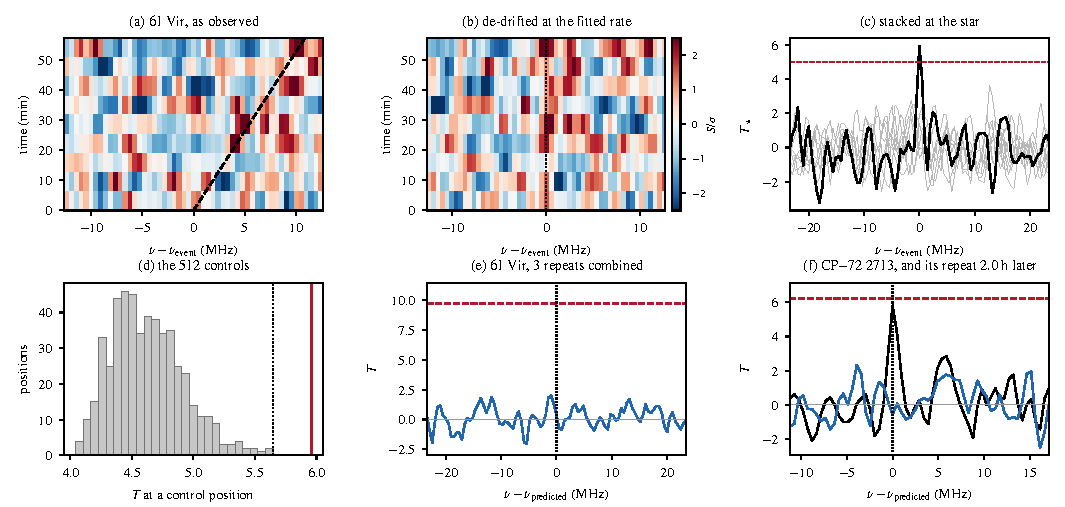
\includegraphics[width=\textwidth]{figures/event_crossings.pdf}
\caption{\textbf{Why this survey reports no confirmed signal although it
produced an interesting event.} \emph{(a)}~The dynamic spectrum at
\EvAStar's position around the crossing at \EvAFreq\,GHz, observed
\EvADate, with the fitted drift of \EvADrift\,Hz\,s$^{-1}$ as the dashed
track; the \EvANInt{} integrations are binned into \EvANBin{} and plotted in
units of each bin's noise. At \EvAFlux$\pm$\EvAFluxErr\,mJy against
\EvARmsInt\,mJy per integration the carrier is \EvAPerIntSig{} standard
deviations in any one of them and is invisible by eye, which is the point:
the event exists only in the \EvADwellMin-minute coherent stack.
\emph{(b)}~The same rows shifted by that drift, which carries the carrier
\EvADriftChan{} channels of \EvAChanwkHz\,kHz across the observation;
\EvANBinPos{} of the \EvANBin{} bins are positive at the marked channel.
\emph{(c)}~The de-drifted stack at the star (black) and at the
\RcNRetCtrl{} control positions with retained dynamic spectra (grey), in
units of its own noise; dashed, the trigger. \emph{(d)}~The same statistic
at each of the \NCtrl{} rank-screen control positions: the star reaches
\EvAT{} (solid) against a highest control of \EvACtrlMax{} (dotted).
\emph{(e)}~The \EvANRep{} other blocks covering that cell in the star's rest
frame, combined, with zero at the \emph{predicted} channel, which the frame
transport moves between epochs; the nearest is \EvANearH\,hours
\EvANearSign{} than the discovery (\EvARepDate), the farthest
\EvASpanD\,days. A persisting carrier would have returned $T=\EvATPers$
(dashed) against \EvATAnyDrift{} present, excluding it at \EvAExcl$\sigma$.
\emph{(f)}~The second event, \EvBStar{} at \EvBFreq\,GHz: its discovery
stack (black) and the same cell \EvBDeepH\,hours later in a block
\EvBDeepRatio{} times deeper (blue), where a persisting carrier would have
given $T=\EvBDeepTPers$ (dashed) against \EvBDeepTObs{} measured. The
inferred isotropic equivalent powers are
$\EvAEirp\times10^{\EvAEirpExp}$\,W at \EvADistPc\,pc and
$\EvBEirp\times10^{\EvBEirpExp}$\,W at \EvBDistPc\,pc.}
\label{fig:event}
\end{figure*}

\begin{table}
\centering
\caption{\textbf{The two events of Fig.~\ref{fig:event}}, the unattributed
crossings whose stellar statistic exceeds all \NCtrl{} control positions of
their own window. Repeat epochs measured are the blocks at which the
predicted stellar-frame cell was read; the indented rows give how many of
those the released catalogue carries and how many blocks it lists as
covering the frequency at all, which differ because the archival extension
is deposited separately. $T_{\rm rep}$ combines the repeat epochs by inverse
variance: it is one cell and one trial, so it may be negative, and it is the
quantity $T_{\rm pers}$ is compared against. The indented readings beneath it
are the largest single epoch and the largest over every drift trial, each a
maximum and so positive on average whatever is there. The exclusion is
$(T_{\rm pers}-T_{\rm rep})/\sqrt{1+(T_{\rm pers}/T_\star)^2}$, the
significance at which two readings of one amplitude disagree, and the last row
is the fraction of the discovery amplitude $S$ still ruled out at the trigger,
$(T_{\rm rep}+5)/T_{\rm pers}$. The radiated power quoted is that implied by
the flux in the peak channel; an unresolved carrier leaves only \HanMed{} of
its power there, so the power actually radiated is
$\times\HanFacBest$--$\times\HanFacWorst$ larger, a factor already inside
$\mathrm{EIRP}_{90}$ and not inside this row.}
\label{tab:cand}
\footnotesize
%% GENERATED by recur_v411.py -- do not hand-edit.
\begin{tabular}{@{}>{\raggedright\arraybackslash}p{0.49\columnwidth}@{~~}r@{~~}r@{}}
\hline
 & 61 Vir & CP$-$72 2713 \\
\hline
Frequency (GHz) & 346.313811 & 344.269746 \\
Channel width (kHz) & 488.28 & 488.28 \\
Drift rate (Hz\,s$^{-1}$) & $+3182$ & $-2056$ \\
$T_\star$ & 5.958 & 5.809 \\
Highest control $T$ & 5.65 & 5.68 \\
Flux density (mJy) & 118.8 $\pm$ 19.9 & 11.3 $\pm$ 2.0 \\
Peak-channel EIRP (W) & $5.1 \times 10^{14}$ & $8.9 \times 10^{14}$ \\
Repeat epochs measured & 3 & 5 \\
\quad in the released catalogue & 3 & 1 \\
\quad catalogue blocks at $\nu$ & 4 & 1 \\
Observed & 2017 May 20 & 2022 Oct 2 \\
Nearest covering epoch & 2017 May 19 & 2022 Oct 2 \\
\quad separation (h) & $-1.97$ & $+2.05$ \\
\quad covering epochs more than a day away & 2 & 4 \\
Longest baseline (d) & 3 & 2 \\
$T$ expected if persistent, $T_{\rm pers}$ & 9.70 & 6.30 \\
$T$ measured, matched drift, $T_{\rm rep}$ & +0.39 & -0.82 \\
\quad largest single epoch & +1.65 & +0.96 \\
\quad maximised over every drift & 2.71 & 3.60 \\
Exclusion, $\sigma_{\rm excl}$ & 4.9$\sigma$ & 4.8$\sigma$ \\
Amplitude still excluded at $5\sigma$ & 0.56 $S$ & 0.66 $S$ \\
Disposition & not confirmed & attributed \\
\hline
\end{tabular}

\end{table}

\begin{table*}
\centering
\caption{\textbf{The threshold crossings of the reserved hold-out}, searched
with the same frozen pipeline and disposed of by the same tests as the
census. $\Delta v_\star$ is the offset from the nearest masked transition in
the star's own frame and $n_{\rm rep}$ the number of covering repeat blocks;
$T_{\rm pers}$ and $T_{\rm rep}$ are as in Table~\ref{tab:ledger}. The one
crossing that is present again is a carbon monoxide line.}
\label{tab:holdout}
\scriptsize
%% GENERATED by holdout_v412.py -- do not hand-edit.
\begin{tabular}{@{}l@{~}l@{~}r@{~}r@{~}l@{~}r@{~~}r@{~}r@{~}r@{~}l@{}}
\hline
Star & block & $\nu_{\rm topo}$ (GHz) & $T_\star$ & line & $\Delta v_\star$ & $n_{\rm rep}$ & $T_{\rm pers}$ & $T_{\rm rep}$ & disposition \\
\hline
HD~285968 & Xdaef5a\_Xdd9b & 230.5081 & 8.642 & CO($2$--$1$) & +8.7 & 4 & 11.6 & +6.71 & attributed; present again \\
HD~14055 & X107376c\_X6126 & 330.7123 & 5.513 & $^{13}$CO($3$--$2$) & +112.6 & 30 & 312.0 & +0.56 & unattributed; does not recur \\
TRAPPIST$-$1 & Xd0e450\_X259b & 346.2454 & 5.326 & SO($9_{8}$--$8_{7}$) & -306.6 & 5 & 11.1 & -0.32 & unattributed; does not recur \\
HD~172555 & X107fa96\_X1300f & 344.6066 & 5.144 & SO($8_{8}$--$7_{7}$) & +251.3 & --- & --- & --- & unattributed; no repeat coverage \\
HD~285968 & Xdb4b9a\_Xa7c & 229.9129 & 5.106 & CO($2$--$1$) & -768.0 & 4 & 11.2 & +0.21 & unattributed; does not recur \\
HR~1010 & Xc6b674\_X23f2 & 346.2301 & 5.044 & SO($9_{8}$--$8_{7}$) & -238.7 & 7 & 25.9 & -0.80 & unattributed; does not recur \\
HD~10647 & Xff99e1\_X9cdf & 345.7059 & 5.017 & SO($2_{3}$--$2_{1}$) & +37.1 & 13 & 142.1 & -0.93 & attributed; does not recur \\
HD~170773 & Xff294f\_X1fb & 345.5597 & 5.001 & SO($2_{3}$--$2_{1}$) & -113.8 & 4 & 59.3 & +1.45 & unattributed; does not recur \\
\hline
\end{tabular}

\end{table*}

%% tab:ledger MOVED to Appendix D (sections/app_J_falsealarm.tex): a
%% full-width 56-row table* worth 0.72 pp of the main text.  Sec. 5.3 and
%% Sec. 5.6 carry the counts and cite it.



\begin{figure}
\centering
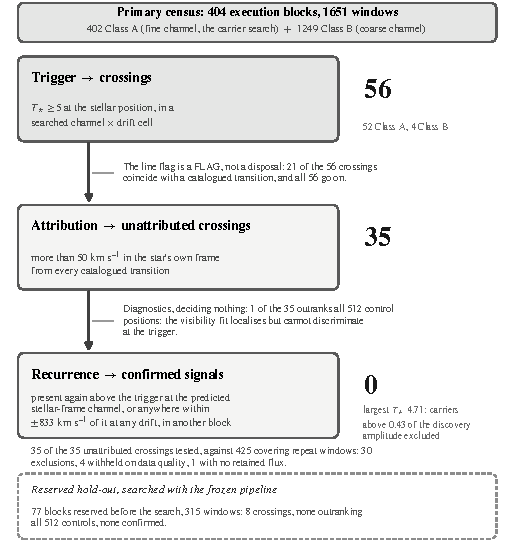
\includegraphics[width=\columnwidth]{figures/chain_v412.pdf}
\caption{The detection logic, with the count surviving each level. Three
levels and no more: a \emph{crossing} is an event requiring investigation, an
\emph{unattributed crossing} is a target for follow-up, and a \emph{confirmed
signal} would be a detection. Coincidence with a catalogued transition is a
flag and not a disposal, so all \CnCross{} crossings continue past it; the
spatial rank and the visibility fit are diagnostics attached to the middle
level and decide nothing. The reserved hold-out is drawn as a separate branch
because a transmitter in it would matter whatever its calibration role. Every
count is read from the ledger and the catalogue, so the figure,
Table~\ref{tab:ledger} and the text cannot disagree.}
\label{fig:chain}
\end{figure}

%% ---------------------------------------------------------------------
%% REQUEST (results owner -> numbers owner).  Eight macros this file uses
%% that the frozen layer does not yet define, all on the adopted
%% trigger-plus-spatial-screen criterion (EirpNinetyMultA = 5.70):
%%   \EirpNinetyWinMedA                      median Class A window, W
%%   \EirpNinetySysLoA \EirpNinetySysMedA \EirpNinetySysHiA
%%                                           per system, best window, W
%%   \EirpNinetyBarnLo \EirpNinetyBarnHi     Barnard's Star, W
%%   \EirpNinetyWolfLo \EirpNinetyWolfHi     Wolf 359, W
%% The \Promote* family (\PromoteMedA, \PromoteSysMedA, ...) is the same
%% quantity on the superseded localisation criterion and is cited nowhere
%% in this file; it is still cited in 03_sample.tex and 07_conclusions.tex,
%% which must move to the names above or the paper will carry two
%% sensitivities again.  \EirpBarnLo/\EirpBarnHi/\EirpWolfLo/\EirpWolfHi
%% are nominal triggers and are no longer quoted here.
%%
%% REQUEST (results owner -> numbers owner).  tab_ledger_v403 must drop
%% nine columns: both visibility-fit epoch groups (Re/sigma, Im/sigma,
%% ctrl, twice), the epoch displacement D, the off-channel column "off",
%% and the "scr" rank flag, whose result is carried by the disposition
%% code.  Eight columns remain: star, block, band, nu, T_star, line, dv,
%% disposition.  \LedgerLegend is replaced by the caption above, so the
%% legend macro is no longer referenced.
%%
%% REQUEST (results owner -> numbers owner).  tab_maskladder.tex now has a
%% home as Table tab:maskladder in this file.  Its fourth column header
%% reads "rank-flagged", a phrase this manuscript has used in both senses;
%% please rename it to "outrank all controls" so the header cannot be read
%% as its own opposite.  The caption states the meaning meanwhile.
%%
%% REQUEST (results owner -> figures owner).  fig:chain MUST BE RE-EMITTED
%% AT SINGLE-COLUMN GEOMETRY.  It is now a \begin{figure} at \columnwidth,
%% not a figure* at 0.98\textwidth, because the section measures 6.0 pp as
%% three full-width floats and 5.0 pp with this one in a column -- the
%% overage was float packing, not words.  chain_v403.pdf is still drawn for
%% full width, so its labels are currently at about half their intended
%% size: PLEASE RE-EMIT FOR ONE COLUMN.  A six-step vertical chain reads
%% better in a column than across a page, so this is the right geometry
%% for it, but the caption, the placement and the artwork must agree and
%% today only two of the three do.  If re-emission is refused, revert this
%% float to figure*/0.98\textwidth and the section is 6.0 pp.
%%
%% REQUEST (results owner -> figures owner).  fig:bpiccontrol.
%%  - GEOMETRY CONFIRMED SINGLE COLUMN.  bpic_control.pdf is 237.6 x 280.7 pt,
%%    i.e. one column wide with the two panels stacked vertically, and the
%%    float is \columnwidth in a \begin{figure}.  Caption and placement
%%    agree; no re-emission at full width is wanted.  Panel (b) gets the
%%    full column width this way, which is what it needs.
%%  - COUNTS I WOULD NOT INVENT.  \NStageOneBpicEb (9) counts the blocks in
%%    which the star outranks every control, so it cannot also count the
%%    points drawn: the ring-wins block is by definition not one of the 9.
%%    The caption therefore says "the 9 ... and one further block" rather
%%    than giving a total.  Four macros would let it say what is drawn:
%%      \BpicPanelNCo     beta Pic CO points in panel (b)        (10)
%%      \BpicPanelNOther  other crossings drawn in grey          (39)
%%      \BpicDvCoLo \BpicDvCoHi   |dv| range of the CO crossings (12-29)
%%      \BpicDvCsLo \BpicDvCsHi   |dv| of the two CS(5-4) crossings
%%    \BpicDvLo/\BpicDvHi existed earlier today and have since been retired.
%%  - COUNTEREXAMPLE NUMBERS, requested and still absent: the ring maximum
%%    (14.13), the stellar statistic (9.68) and the number of the \NCtrl
%%    controls above the star (6) in the ring-wins block.  When they exist
%%    the caption should name that block instead of gesturing at it.
%%
%% REQUEST (results owner -> integrator).  Labels and floats deleted from
%% this file, with the files that still reference them:
%%   sec:linecost     -> sec:bpicval   (06_discussion, app_F, app_I, app_K)
%%   sec:repairedstat -> app:v409      (08_backmatter, app_A, app_M)
%%   eq:tunif         no longer defined anywhere (app_L cites it)
%%   tab:crossdelta   float deleted with the revision-history material;
%%                    app_M_repaired.tex still cites it
%%   tab:clustv409    float deleted; nothing else cites it
%%   fig:ledgervis    no longer cited (float lives in app_K)
%%   tab:hosts        no longer cited from here
%%   app:etacrvrecur  no longer cited from here (app_M still cites it)
%% ---------------------------------------------------------------------
